\lstset{
    numbers=left, 
    numberstyle= \tiny, 
    keywordstyle= \color{ blue!70},%设置关键字颜色
    commentstyle= \color{red!50!green!50!blue!50}, %设置注释颜色
    frame=shadowbox, % 阴影效果
    rulesepcolor= \color{ red!20!green!20!blue!20} ,
    escapeinside=``, % 英文分号中可写入中文
    xleftmargin=2em, %距离左边界2em
    aboveskip=1em,
    framexleftmargin=2em,
    basicstyle=\ttfamily,
    columns=fullflexible,%可以自动换行
    linewidth=1\linewidth, %设置代码块与行同宽
    breaklines=true,%在单词边界处换行。
    showstringspaces=false, %去掉空格时产生的下划的空格标志, 设置为true则出现
    breakatwhitespace=ture,%可以在空格处换行
    escapechar=`%设置转义字符为反引号
}
\chapter{日常计划}
\section{2024年度}
\begin{itemize}
    \item AptamerCOVID-19 投出去 (目前文章在周那里修改)
    \item SM3CLCOVID-19 投出去 (投稿至JPCL)
    \item * VEGF环肽 完成投稿 (最重要)(目前正在绘图,写文章,9月底之前弄完)
    \item * 深度学习算法根据结构优化Aptmaer 主体工作完成 (最重要)(还没搞,12月底之前主体部分弄好)
    \item * 靶向PKR的环Aptamer优化设计 (最重要)(还没做,明年3月底之前主体部分弄好)
    \item \textbf{下面都是合作的,都乱七八糟的,优先级最后}
    \item (合作)张兴老师二甲双胍 投出去 (目前还在修)
    \item (合作)药学院滕鹏老师课题 做完
    \item (合作)浙一 白雪莉老师课题 完成投稿 (垃圾课题,垃圾课题组,再也不给他们做MD了,再做我是狗。)
    \item (合作)南通大学 李霞老师课题 做完 (实验那边出了问题)
    \item (合作)黄力全老师,做完
\end{itemize}
\chapter{已发表文章}
\chapter{待解决的重要科学问题}
\section{Q1: 环肽的透膜性}
目前,每年都有FDA批准的环肽药物,但是目前开发的环肽药物大多都仍有未被解决的一些问题,
目前所有上市的环肽大分子都是无法口服使用的,因为环肽的透膜性方面还有一定的问题未被解决。
所以可以采用MD模拟的方式研究环肽的透膜性质。
\section{Q2: 生物分子结合动力学}
两个生物大分子结合时候,在具体的结合过程中一定会有优先结合与滞后结合的part区别,可以挑一个好的研究体系
对两个生物分子之间的结合进行详细的MD模拟,通过大量的模拟两者之间的结合过程,然后找出两者之间结合时候的
动态过程,确定主要的驱动力以及次要的带动力,然后根据他们的结合时候的动态机制进行合理改造从而进一步增强
这个生物分子结合过程时候的动力学性质。进一步增强结合亲和力。
\section{Q3: 将强而无活性的结合分子转化为功能有效的调节剂分子}
在有些体系当中,并不是结合亲和力越高的分子就一定能够发挥预期的功能,达到治疗的效果。
所以将结合亲和力强的分子转换为发挥功能性的分子是很重要的。其中一个有效的方法就是使用PROTAC。
在结合亲和力强的分子上连接上能使得蛋白降解的降解剂就是一个很好的做法,所以一个很好的直的研究的课题就是
从现有的文献中寻找一些结合亲和力很强的但是功能上没有活性的biobinder,然后连上降解剂看看效果。然后优化优化。
\section{Q4:二甲双胍作用机理的模拟研究}
二甲双胍是一种非常重要的药物,并且研究也报道了它的很多的作用效果。可以想想怎么能对二甲双胍的作用机理展开一些计算模拟。
\section{Q5:长新冠的相关研究,以后不做新冠了,这个切掉}
华尔街日报:“长新冠”导致约100万美国人失业,360万人生活发生重大变化。
长新冠的相关链接:https://mp.weixin.qq.com/s/houMhmt1PwdI1lKZWIhT6A。
\section{Q6:REMD+CMD+MSM进行构象转变的机制研究}
使用短时间的REMD在每一个低点local进行代表性的构象采样(可能需要改进算法,每个低点只需要一个代表性的构象就可以。交换到一个新的低点的打上一个标签之后就不要再在这个地方进行采样了)。
然后取出代表性构象进行长时间的常规动力学模拟,然后使用多条轨迹应用MSM进行构象变化的机制研究。
\section{Q7:模拟退火+CMD+MSM进行构象转变的机制研究}
与Q6类似,使用模拟退火对蛋白局部稳定结构进行采样。然后取出代表性构象进行长时间的常规动力学模拟,然后使用多条轨迹应用MSM进行构象变化的机制研究。
或者别搞这么麻烦了,就直接使用高温分子动力学模拟好了(就将耦合温度修改下就行)。
\section{Q8:深度学习中的对比学习应用于FEP计算数值的正负当中}
https://mp.weixin.qq.com/s/n3brg8\_VRSr\_ET6K8FlYtw
\section{Q9:想想办法将现有的生物体系中的蛋白和核酸借助一些方式在体内组装成能够发射信号的生物机器人}
\section{Q10:看蛋白核酸晶体结构时候发现核酸的结合位点形状有很大的特色,所以可以借鉴现在的3D识别的AI技术用于预测蛋白中核酸的结合位点}
\section{Q11:long noncoding 核酸的构象采样,可以采用3d碎片拼接的方式进行长链RNA三维构象空间的广泛采样,可以做成一个程序}
\section{Q12:一个非常值得研究的课题,数据量于模型复杂度之间的关系,一般比例是多少的时候预测性能会比较好}
\chapter{博论}
\section{时间安排}

有时间的时候需要慢慢开始写博士论文了。
\newline \noindent 目前想写的博论的主要内容有:接续之前的D3Similarity和D3AI-CoV模块,第一章写一下pan-CovBoost的方法以及应用。
\newline \noindent 第二章写一下物理驱动的MD模拟(FEP)+数据驱动的深度学习模型用于RNA 适配体的优化开发的方法。
\newline \noindent 第三章写一下靶向新冠病毒适配体的开发。
\newline \noindent 第四章写一下将上述的所有方法都集合在了网站里面以便使用。
\chapter{专题研究}
\section{冠状病毒研究专题}
\subsection{文献阅读}
\section{呼吸蛋白研究专题}
\section{核酸相关研究专题}
\subsection{文献阅读}
\noindent * (nature methods/2024) Geometric deep learning of protein-DNA binding specificity 

\chapter{自己主导的课题}
\section{D3Similarity}
\section{D3AI-Cov}
\section{靶向SARS-CoV-2 S蛋白适配体优化设计课题}
\subsection{整体文章脉络}
\noindent\textbf{该文章的落脚点在于aptamer drug design,弱化一下COVID-19。亮点在于长序列aptamer的快速设计和重大疾病的响应;效果堪比抗体,可以替代抗体发挥作用}
\newline\noindent 整篇文章的时态,abstract和introduction使用的是一般现在时,其他使用的都是一般过去时。
\newline\textbf{Introduction}
\newline\indent Para1: Aptamer很好,很有用,临床应用意义非凡。
\newline\indent Para2: 我们这篇文章的目的何在?奠定本文方法为主,应用为辅的基调。写一下目前我们想做的事情所遇到的困难以及我们解决困难的办法。也着重写一下相较于之前工作的一些进步的地方。
\newline\indent Para3: 引出新冠RBD的适配体的案例。着重强调一下目前的RBD抗体的一些缺陷然后引出我们为什么要做RBD的适配体。
\newline\indent Para4: 详细的讲一下Figure1,Figure1是对这篇工作的一个通览。
\newline\noindent\textbf{Results}
\newline\indent Para1: 结合模式的分析,具体的细节全部要放在Method中,这里主要是对结果的分析以及具体的数值分析。
\newline\indent Para2: 与抗体的效果进行比较,这里要详细的写,这个点是这篇文章的亮点所在。
\newline\indent Para3: In silico design,这部分是这篇文章的重点所在,要详细的写,要将具体的数值都体现出来。
\newline\indent Para4: 实验验证和分子机制。多写以及详细的分析。
\subsection{Paper-Figures}
\noindent FS2: RMSD曲线图和两个构象叠合图。
RMSD曲线图脚本:do202405091802.py 
\subsection{Paper-Writing}
\noindent\textbf{(1) 新冠抗体的ADE(Antibody-dependent enhancement)效应}
\newline\indent 已有研究表明,抗SARS-CoV-2抗体可能通过ADE效应来加剧COVID-19症状。
ADE的两种机制:(1) 一些病毒特异性的非中和抗体与病毒互作,沾染有病毒的抗体的Fc段与能表达FcR的一些细胞(如单核细胞和巨噬细胞)互作之后会将病毒连带着侵染这些正常细胞,从而加剧感染。(2) 抗体依赖的过多FC介导的效应功能和免疫复合物导致疾病加剧并发生免疫反应,通过启动一个强大的免疫级联来增强呼吸道疾病。
\newline\noindent 参考资料
\begin{itemize}
    \item \href{https://zhuanlan.zhihu.com/p/677496719#:~:text=%E7%96%AB%E8%8B%97%E5%92%8C%E6%8A%97%E4%BD%93%E8%8D%AF%E7%89%A9%E7%9A%84%E4%B8%80%E4%B8%AA%E4%B8%BB%E8%A6%81%E7%9B%AE%E6%A0%87%E6%98%AF%E4%BA%A7%E7%94%9F%E6%8A%97%E4%BD%93%EF%BC%8C%E9%80%9A%E8%BF%87%E9%98%BB%E6%96%AD%E7%97%85%E6%AF%92%E4%B8%8E%E5%85%B6%E7%BB%86%E8%83%9E%E5%8F%97%E4%BD%93%E7%BB%93%E5%90%88%E6%88%96%E4%B8%8E%E7%BB%86%E8%83%9E%E8%86%9C%E7%9A%84%E8%9E%8D%E5%90%88%E4%BD%9C%E7%94%A8%E9%98%BB%E6%AD%A2%E6%96%B0%E5%86%A0%E7%97%85%E6%AF%92%EF%BC%88SARS-CoV-2%EF%BC%89%E8%BF%9B%E5%85%A5%E7%BB%86%E8%83%9E%E3%80%82%20%E7%84%B6%E8%80%8C%EF%BC%8C%E5%9F%BA%E4%BA%8E%E6%8A%97%E4%BD%93%E7%9A%84%E7%96%AB%E8%8B%97%E5%8F%8A%E8%8D%AF%E7%89%A9%E7%96%97%E6%B3%95%E7%9A%84%E4%B8%80%E4%B8%AA%E6%BD%9C%E5%9C%A8%E9%9A%9C%E7%A2%8D%E6%98%AF%EF%BC%9A%E6%8A%97%E4%BD%93%E4%BE%9D%E8%B5%96%E6%80%A7%E5%A2%9E%E5%BC%BA%EF%BC%88Antibody%20dependent%20enhancement%EF%BC%8CADE%EF%BC%89%E6%95%88%E5%BA%94%E3%80%82,%E5%B7%B2%E6%9C%89%E7%A0%94%E7%A9%B6%E8%A1%A8%E6%98%8E%EF%BC%8C%E6%8A%97SARS-CoV-2%E6%8A%97%E4%BD%93%E5%8F%AF%E8%83%BD%E9%80%9A%E8%BF%87ADE%E6%95%88%E5%BA%94%E6%9D%A5%E5%8A%A0%E5%89%A7COVID-19%E7%97%87%E7%8A%B6%E3%80%82%20ADE%E5%8F%91%E7%94%9F%E6%9C%BA%E5%88%B6%20%E6%89%80%E8%B0%93%E7%9A%84ADE%E6%95%88%E5%BA%94%E6%98%AF%E6%8C%87%E6%9F%90%E4%BA%9B%E7%97%85%E6%AF%92%E7%89%B9%E5%BC%82%E6%80%A7%E6%8A%97%E4%BD%93%20%28%E4%B8%80%E8%88%AC%E5%A4%9A%E4%B8%BA%E9%9D%9E%E4%B8%AD%E5%92%8C%E6%8A%97%E4%BD%93%29%E4%B8%8E%E7%97%85%E6%AF%92%E7%BB%93%E5%90%88%E5%90%8E%EF%BC%8C%E7%BB%93%E5%90%88%E4%BA%86%E7%97%85%E6%AF%92%E7%9A%84%E6%8A%97%E4%BD%93%E5%8F%AF%E9%80%9A%E8%BF%87%E5%85%B6%E6%8A%97%E4%BD%93Fc%E6%AE%B5%E4%B8%8E%E6%9F%90%E4%BA%9B%E8%A1%A8%E9%9D%A2%E8%A1%A8%E8%BE%BEFcR%E7%9A%84%E7%BB%86%E8%83%9E%E7%BB%93%E5%90%88%E4%BB%8E%E8%80%8C%E4%BB%8B%E5%AF%BC%E7%97%85%E6%AF%92%E8%BF%9B%E5%85%A5%E8%BF%99%E4%BA%9B%E7%BB%86%E8%83%9E%E3%80%82%20%E4%B8%80%E8%88%AC%E8%AE%A4%E4%B8%BA%EF%BC%8C%E5%9C%A8%E4%BD%BF%E7%94%A8%E7%96%AB%E8%8B%97%E6%88%96%E6%8A%97%E4%BD%93%E6%B2%BB%E7%96%97%E7%97%85%E6%AF%92%E6%84%9F%E6%9F%93%E6%97%B6%EF%BC%8C%E5%A6%82%E6%9E%9C%E4%BA%A7%E7%94%9F%E7%9A%84%E6%8A%97%E4%BD%93%E6%95%88%E4%BB%B7%E4%B8%8D%E9%AB%98%E6%88%96%E8%80%85%E9%9D%9E%E4%B8%AD%E5%92%8C%E6%8A%97%E4%BD%93%E6%97%B6%EF%BC%8C%E5%B0%B1%E4%BC%9A%E4%BA%A7%E7%94%9FADE%E6%95%88%E5%BA%94%E3%80%82}{抗体依赖性增强(Antibody dependent enhancement,ADE)效应}
\end{itemize}
\subsection{RBD和适配体对接}
\noindent (1) RBD单体的动力学模拟,聚类选取RBD的稳定构象进行对接。  
RBD的pbc处理,RMSD计算和聚类脚本:do202405091645.sh
\subsection{聚类之后代表性RBD-适配体复合物的分子动力学模拟}
\noindent (1) 复合物的pbc处理,RMSD计算和聚类脚本:脚本参考do202405091645.sh,将居中原子编号修改成距离复合物中心近的原子编号。
\section{深度学习+FEP靶向新冠病毒3CL的小分子优化设计课题}
\subsection{整体文章脉络}
大致故事:使用AI模型进行了预测,发现有两个负的,还有一些紧跟排在后面的。然后又对cl原子替换的地方做了预测。可以分批次的进行AI预测以及FEP计算,没必要一下子预测。
\subsection{Paper-Figures}
目前图的逻辑还是有问题
\subsection{Paper-Writing}
\noindent 目前初稿是发给周老师,但是可能需要再想想写个dicussion。
\subsection{片段拼接生成小分子库}
\noindent\textbf{= 将Chembl化合物碎片化生成碎片字典库}
\newline\indent 将Chembl数据库下载下来,清理数据获得只含有化合物编号以及对应SMILES的文件,再将化合物碎片化,脚本:/script/深度学习FEP靶向新冠病毒3CL的小分子优化设计课题/ generatefragmentdict202403111549.py job202403111558.sh
\newline\indent 整理所有碎片,去重,统计并生成可投入使用的小分子碎片字典库:/script/深度学习FEP靶向新冠病毒3CL的小分子优化设计课题/ cleanfragmentdict202403111629.py
\newline\noindent\textbf{= 针对先导化合物中的某个基团进行片段替换生成小分子库}
\newline\indent 生成小分子库的脚本:/script/深度学习FEP靶向新冠病毒3CL的小分子优化设计课题/ generatemollibrary202403121631.py
\subsection{AI模型用于ddg预测}
\noindent\textbf{= 五折交叉验证}
\newline\noindent == SMILES正则化
\newline\indent 正则化脚本:/script/深度学习FEP靶向新冠病毒3CL的小分子优化设计课题/ standardsmiles202403042210.py
\newline\noindent == 数据分割
\newline\indent 五折交叉验证数据生成脚本:/script/深度学习FEP靶向新冠病毒3CL的小分子优化设计课题/ datasplit202403042225.py
\newline\noindent == 五折交叉训练
\newline\indent 训练脚本:/script/深度学习FEP靶向新冠病毒3CL的小分子优化设计课题/ ddgpredict5fold202403051628.py
\newline\noindent == 五折交叉结果分析
\newline\indent 获取每折MSE,皮尔森系数和一致性指数的脚本:/script/深度学习FEP靶向新冠病毒3CL的小分子优化设计课题/ getrt202403051643.sh
\newline\noindent\textbf{= 整合所有数据训练用于实际预测的模型}
\newline\noindent == 将所有的活性数据形成pairs
\newline\indent 输入数据的格式是两列(一列是SMILES,一列是活性数值。)。将该数据一整个形成pairs。脚本:/script/深度学习FEP靶向新冠病毒3CL的小分子优化设计课题/ datapreparation202403042122.py
\newline\noindent == 模型训练
\newline\indent 训练脚本:/script/深度学习FEP靶向新冠病毒3CL的小分子优化设计课题/ ddgpredictall202403042151.py
\newline\indent 服务器128上提交脚本:/script/深度学习FEP靶向新冠病毒3CL的小分子优化设计课题/ job202403051433.sh
\newline\noindent\textbf{= 外部输入数据预测}
\newline\indent 与先导化合物形成pairs输入的脚本:/script/深度学习FEP靶向新冠病毒3CL的小分子优化设计课题/ makeinputforpredict202403121637.py
\newline\indent 外部预测脚本:/script/深度学习FEP靶向新冠病毒3CL的小分子优化设计课题/ ddgpredictout202403051626.py
\newline\indent 多模型集成进行外部预测脚本:/script/深度学习FEP靶向新冠病毒3CL的小分子优化设计课题/ ddgpredictout202403122159.py
\subsection{小分子FEP计算}
\subsection{5个候选化合物与3种冠状病毒主蛋白酶模拟展示pan效应}
\noindent = 使用charmm-cgenff力场模拟动力学模拟示例:这次采用的是使用charmm-gui的solution builder对复合物进行建模。
(1)首先在pymol中对配体进行编辑并保存为mol2格式文件。(2)将配体的mol2文件上传charmm-gui的ligand模块生成参数。
(3)将ligandrm.pdb中的信息对complex.pdb中的配体信息进行替换,保证原子名称和数目的一致性(因为该配体中都含有氯原子会产生孤对电子,所以将LPH的一行删除)。
(4)将力场文件中的rtf文件的LPH行都删除,并且要将CL的电荷要+0.05,不然charmmgui会报错。
(5)然后上传charmmgui生成gmx能运行的文件。
(6)结果跑了一些发现使用charmm力场跑的MD配体和蛋白结合不太稳定。
\newline = 使用14sb-gaff力场模拟动力学模拟示例。脚本:build202409131836.sh
\newline = 对蛋白backbone和配体三个原子增加位置限制的模拟文件。脚本:respos202409151839.sh
\newline = pbc处理,rmsd计算,contact计算的脚本文件:pbc202409231018.sh   contact202409231018.py
\subsection{待做}
\noindent\textbf{(1)} 该课题的临时脚本集合:/script/深度学习FEP靶向新冠病毒3CL的小分子优化设计课题/tmp/ utility202403111443.py
\section{接着pan-CovBoost,应用MD+对比学习+FEP进行新冠肺炎分子亲和力优化}
\subsection{temp}
\noindent \textbf{= 想到的课题的思路}
\newline(1)使用RCSB中所有的冠状病毒主蛋白酶和木瓜样蛋白酶的晶体结构。使用MD提取晶体三维结构中的总体的互作或者局部口袋/亚基团的互作进行对比学习,
然后再结合一些FEP的数据增强的数据。完善对比学习用于推荐化合物。
\newline(2)
\section{靶向VEGF的环肽优化设计课题}
\subsection{背景}
\noindent \textbf{reference}: Structural and ITC Characterization of Peptide-Protein Binding: Thermodynamic Consequences of Cyclization Constraints, a Case Study on Vascular Endothelial Growth Factor Ligands
\newline \indent Peptides have many strengths: high target selectivity; good efficiency; safety, and tolerability.
\newline \indent Peptides have many weaknesses: a short plasma half-life; chemical and phyical instabilities and low membrane permeability.
\newline \indent Cyclic peptides have some strengths: reduce susceptibility to proteolysis; stablize their bioactive form and improve both affinity and specificity.
\newline \indent We assumed that it must be possible to gain affinity by stablizing the peptide structure observed in the bound state through pre-folding of the C-terminal part into the bioactive helical conformation.
\newline \indent The structure-activity relationship demonstrated that neither the protein nor the peptide boinds in a conformation corresponding to its energy minimum, and that the peptide must fold upon binding. 
\newline \indent It is confirmed the presence of helical structure in the C-terminal segment (residues P10-15) of the bicyclic peptides 1c, 2c and 3c. However, the monocyclic and 4c peptides have random structures in the C-terminal segment.
\newline \indent The N-terminal part of all the eight peptides were similar and unaffected by the differences in the C-terminal part.
\newline \indent 2c and 3c only can be clustered into a single cluster. Others have many clusters, showing a large flexibility.
\newline \indent The free peptides did not exist as a single conformation in solution.
\newline \indent There are two symetrical VEGF binding sites in crystal structure, one was partially occupied by a peptide molecule, the other site being inaccessible by steric hindrance.
\newline \indent 总结:NMR的分析结果显示自由态的肽在溶液中的构象多样并且相互之间随机变化,在结合状态时候则倾向于形成唯一确定的构象。
通过NMR对自由态和结合态的肽结构进行分析发现结合时候的肽结构与结合时候观察到的自由状态时候的最低能状态是不对应的。
\subsection{整体文章脉络及提纲}
\noindent = 文章脉络
\newline\indent (1) 首先每个位点选取代表性的不同类型氨基酸进行初步FEP计算。
\newline\indent (2) 进行少个的预测。
\newline\indent (3) 预测后再FEP计算,随着数据增加,预测和计算结果的一致性升高。
\newline\indent (4) 计算完成一多半之后,其他的只用预测的数据,不用进行fep计算。
\newline\indent (5) 预测双突,首先采用采样方式遍历所有位点,并使用单突数据初步预测双突,结果差强人意。然后加入双突预测结果之后,再进行其他的双突预测,发现一致性较高。
\newline\indent (6) 从双突出发排列三突,从三突出发排列四突,从四突出发排列五突。以同样的方式预测和计算三突,四突和5突。 
\newline\indent (7) 起一个好听的名字,边走边调整的自由能路径搜索策略。 
\newline\noindent = 提纲
\newline\indent == Title:结合机器学习和FEP进行自由能路径搜索用于靶向VEGF的双环肽开发
\newline\indent == Introduction:第一段:照着陈玲玲的nature biotech写环肽的重要性和优势;
第二段:写VEGF在疾病发展中的重要性以及现在的药物发展现状;
第三段:
第四段:
\newline\indent == Results:
\newline\indent === 第一部分:环肽自由能landscape最小值路径的自动搜索。
\newline\indent === 第二部分:机器学习引导,束搜索策略,FEP计算用于VEGF双环肽抑制剂的优化设计。
\newline\indent === 第三部分:VEGF和双环肽的MD;FEP与实验的吻合程度;以及丙氨酸扫描的结果,选出可用于进一步优化设计的hotspots。
\newline\indent === 第四部分:不同类型氨基酸FEP扩增数据集构建机器学习模型;机器学习预测;单突的所有数据。以及机器学习预测和真实FEP计算值之间的相关性。
\newline\indent === 第五部分:对单突的结果进行双突的束搜索MD,并使用单突组成的机器学习模型预测,排名靠前的进行FEP计算,其中双突的可以分成两次进行机器学习预测和FEP计算,
表征出来单突的机器学习模型在起初的双突预测时候的准确度并不高,随着双突FEP数据的增加,机器学习模型的预测准确度在提高。
\newline\indent === 第六部分:对三突-五突使用同样的机器学习-FEP的综合方法进行结合自由能计算。发现临近的突变可能会受到协同效应的影响,但是MD也是可以表征出来的。
\newline\indent === 第七部分:最好能进行一定的实验验证以及机制解析,最好分成两次分析,实验数据与机器学习预测值的相关性分析以及实验数据与FEP计算值的相关性分析。
\newline\indent == Discussion and Conclusion:
\newline\indent == Methods:
\subsection{Paper-Figures}
\noindent \textbf{= 该课题绘图配色}
\newline 该课题的绘图配色如\autoref{fig:img202407111032},\autoref{fig:img2024071110321},\autoref{fig:img202407111033},\autoref{fig:img2024071110331}和\autoref{fig:img202407111044}所示。
\newline 最终选用的色彩主要有:
\begin{figure}[htbp]
    \centering
    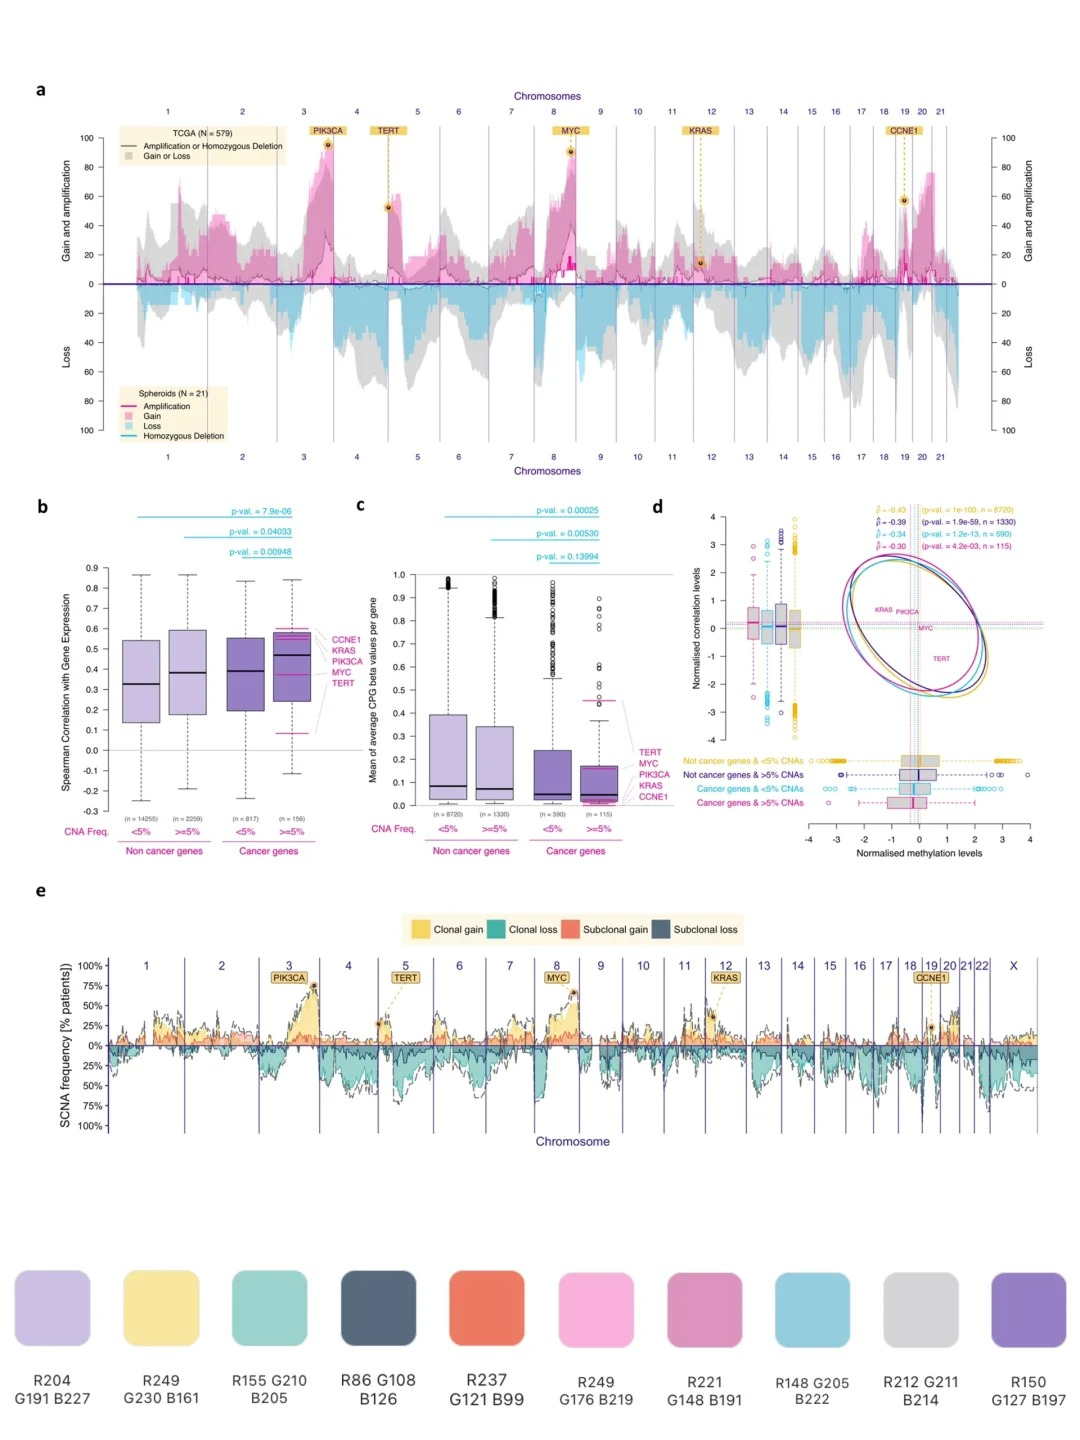
\includegraphics[width=.5\linewidth]{cyclicVEGF/img202407111032.jpg}
    \caption{\label{fig:img202407111032}绘图配色}
\end{figure}
\begin{figure}[htbp]
    \centering
    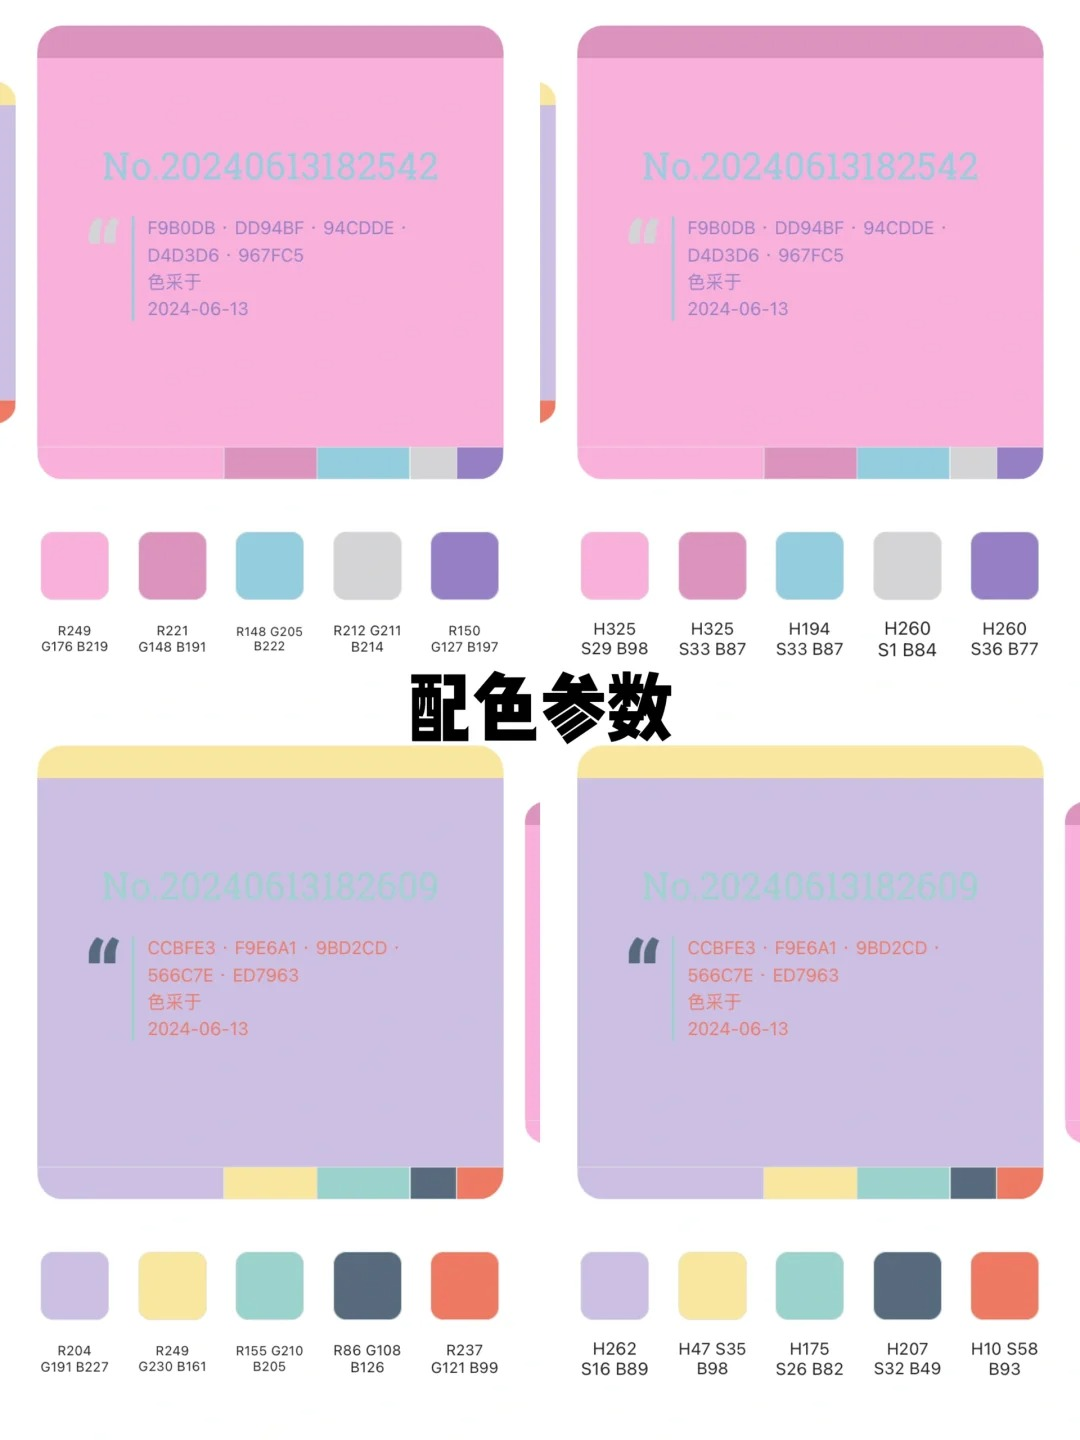
\includegraphics[width=.5\linewidth]{cyclicVEGF/img2024071110321.jpg}
    \caption{\label{fig:img2024071110321}绘图配色}
\end{figure}
\begin{figure}[htbp]
    \centering
    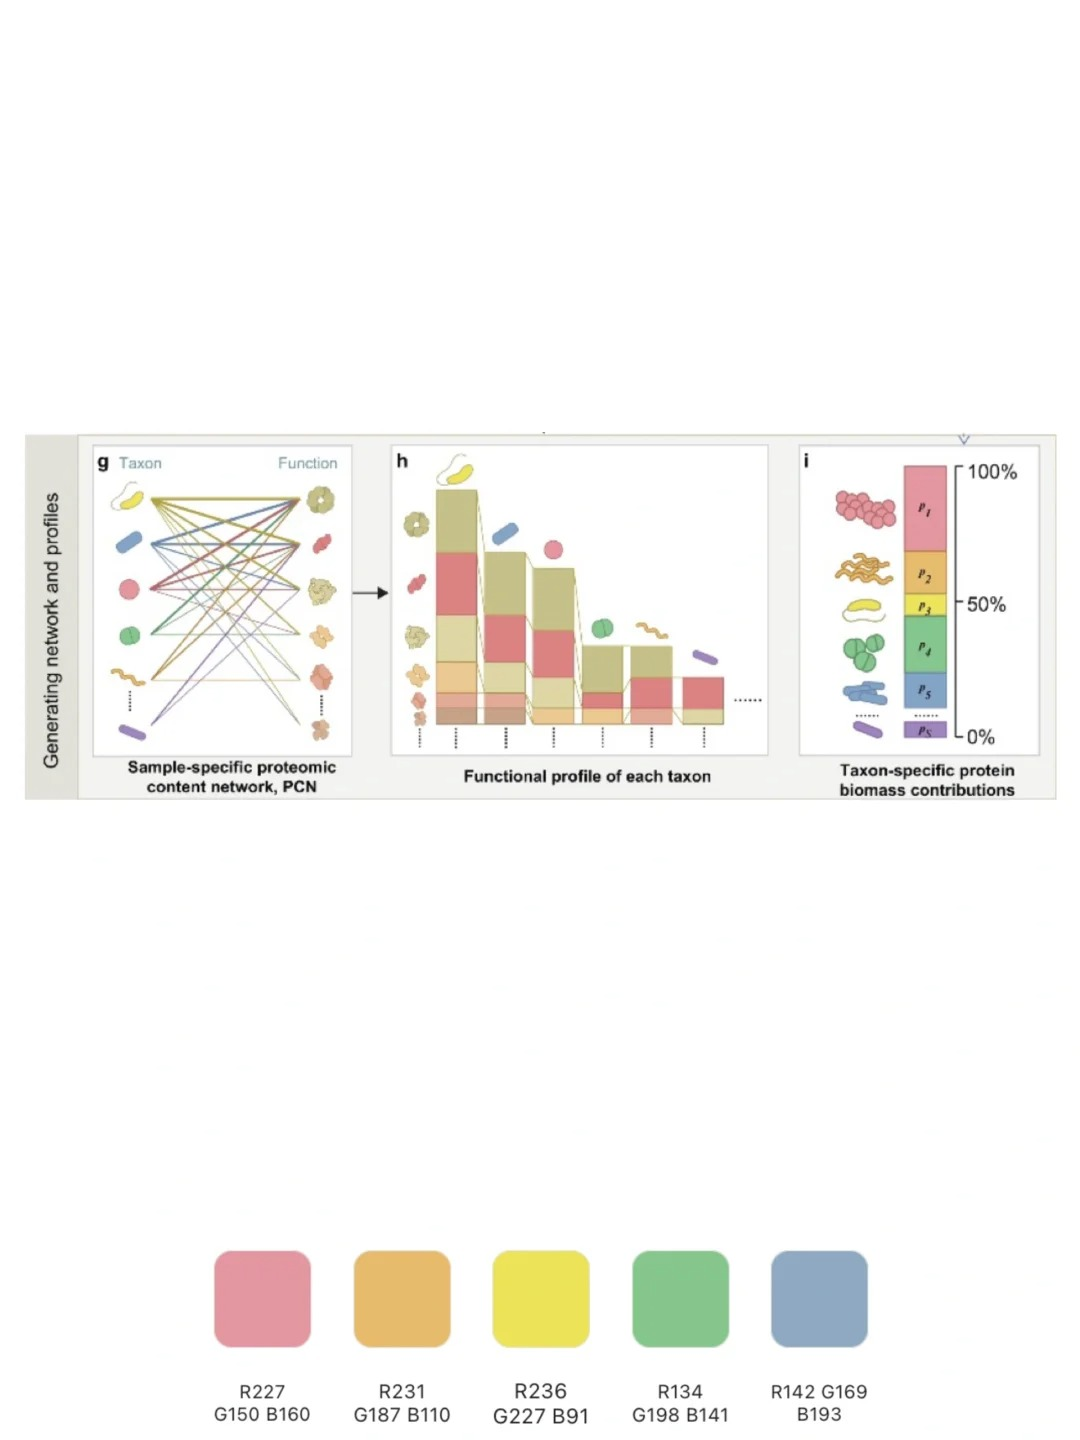
\includegraphics[width=.5\linewidth]{cyclicVEGF/img202407111033.jpg}
    \caption{\label{fig:img202407111033}绘图配色}
\end{figure}
\begin{figure}[htbp]
    \centering
    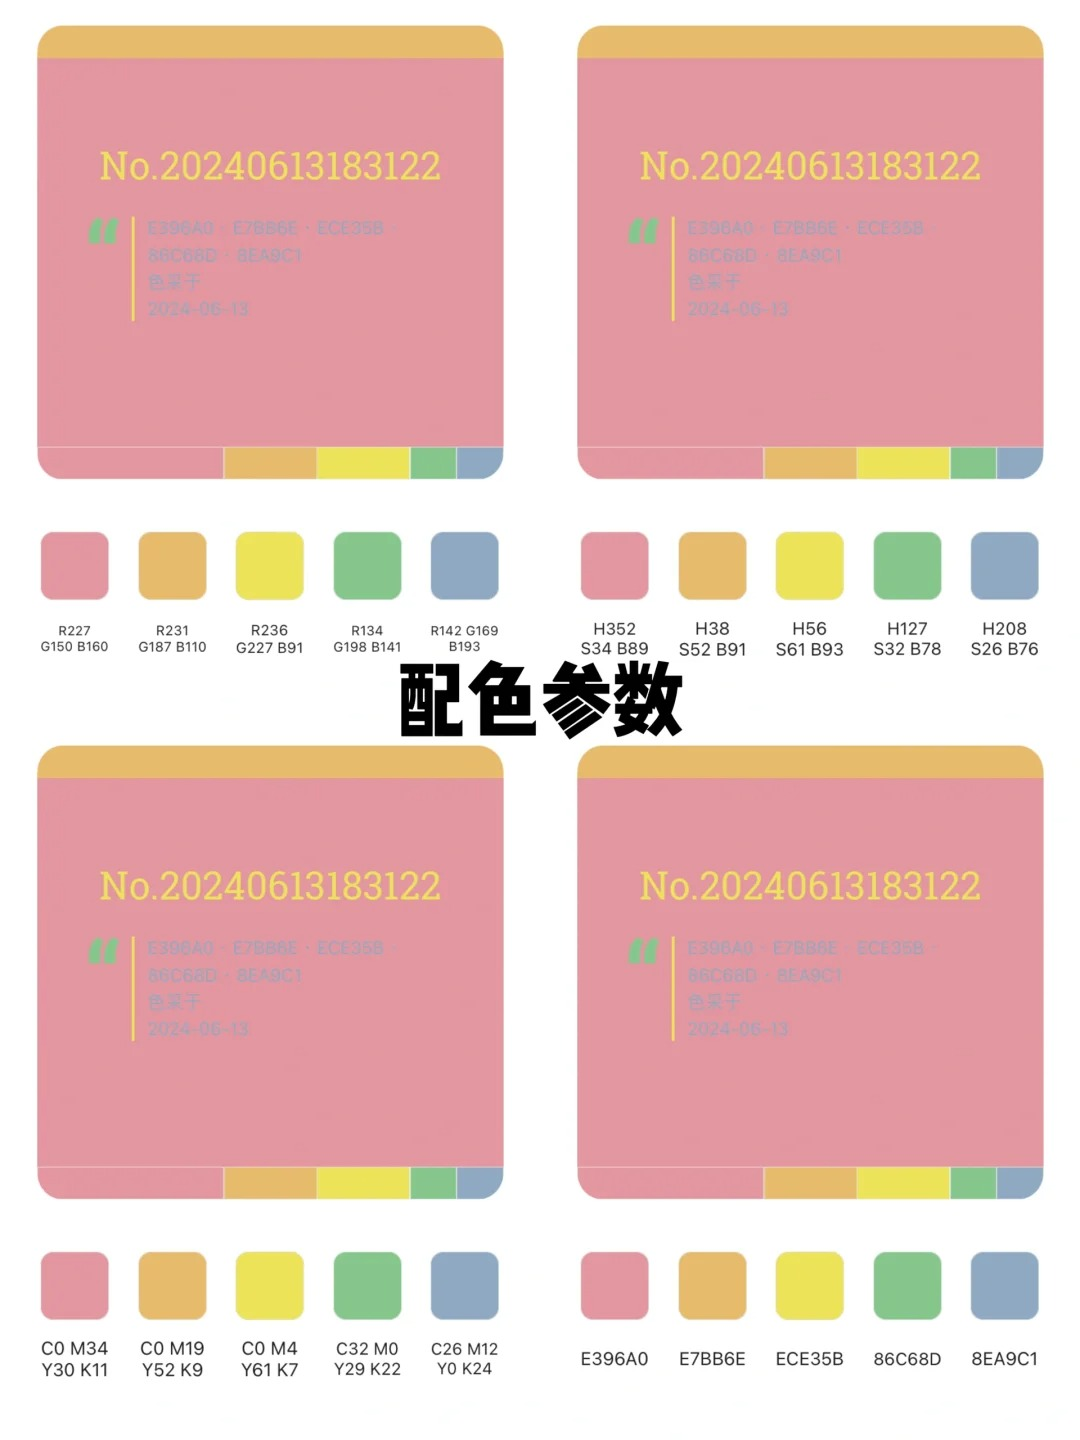
\includegraphics[width=.5\linewidth]{cyclicVEGF/img2024071110331.jpg}
    \caption{\label{fig:img2024071110331}绘图配色}
\end{figure}
\begin{figure}[htbp]
    \centering
    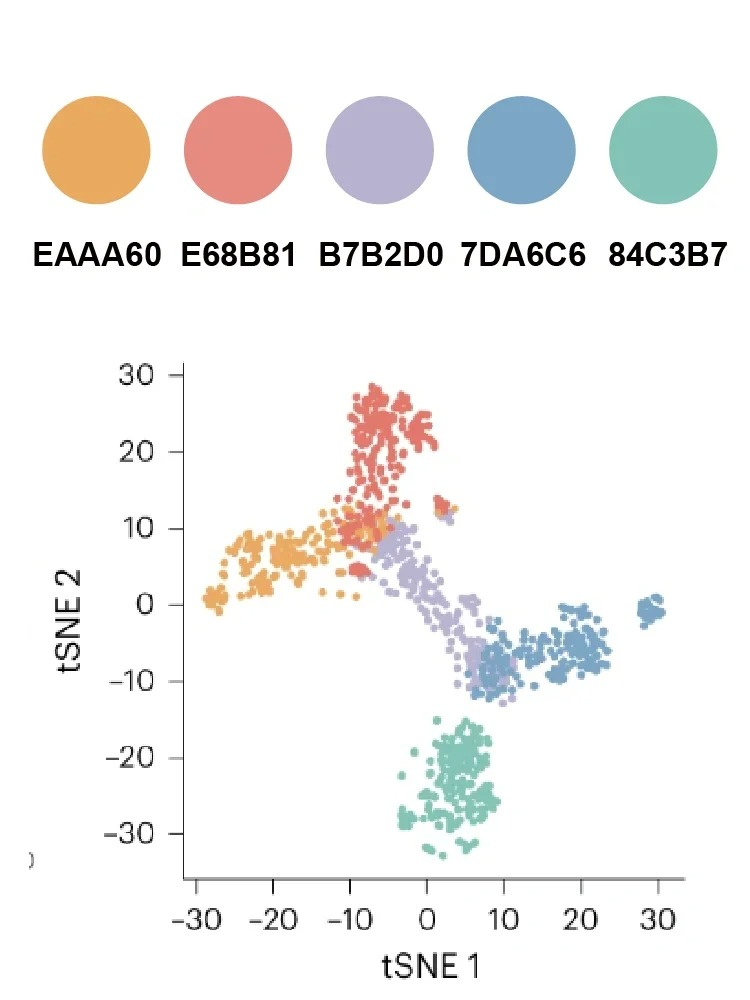
\includegraphics[width=.5\linewidth]{cyclicVEGF/img202407111044.jpg}
    \caption{\label{fig:img202407111044}绘图配色}
\end{figure}
\newline \noindent\textbf{= 绘图纲要}
\newline\noindent\textbf{F1}: (A) 画一张可以体现出VEGF重要调控作用的信号通路的相关图(这个照着NC上面的绘制);
(B) 可以再画一张使用抑制剂抑制VEGF和VEGFR结合从而进行疾病治疗的机制图;
(C) VEGF-VEGFR互作的结构示意图;
(D) VEGF和双环肽互作的结构示意图;
(E) 画一张结合ML和FEP进行自由能landscape构建的框架简图。(类似PNAS的Fig.2A);
(F) 再画一张ML和FEP和实验数据结合起来的图。(类似PNAS的Fig.2C的图)。
(G) 或许图1可以分成两张图??
\newline\textbf{F2}: (A) 画一个VEGF和双环肽结合的结构图,然后放在以圆珠子的多肽形式显示双环肽的序列组成;
(B) 放一下MD中的VEGF和双环肽的相互作用图谱(这个还不知道应该怎么绘制),或者其他之类的,目的是体现MD和关键的一些残基以及可被改造的一些残基;
(C) 放一下丙氨酸扫描的图片以及与实验的吻合程度的图片,这张图再想想看是用一张小图还是两张小图进行表示;
(D) 放一张每个残基的RMSF的图??
\newline\textbf{F3}: (A) 单突的各种类型的FEP的计算数据展示;
(B) 单突MD数据以及FEP数据的机器学习模型构建;
(C) 其他单突的预测以及FEP计算值的相关性程度。
(D) 总结单突时候每个位点的偏好性。
(E) 将每个位点的最优的残基显示出来并且和之前的做一下对照(突变之前的使用透明的,突变之后亲和力变好的使用实体的)。
(F) 绘制一张有关氨基酸性质的图片,方便更有效的探索多肽的空间,使用小量的计算探索更广阔的肽空间。
\newline\textbf{F4}: (A) 每个位点的计划突变的排名靠前的残基;
(B) 显示第一轮的机器学习模型预测结果和计算值之间的相关性。(该轮预测的时候使用的是单突的预测双突的) ;
(C) 第二轮的预测结果;
(D) 第三轮的预测结果;
(E) 双突的一些总结。
\newline\textbf{F5}: 三突,四突和五突的图片制作。
\newline\textbf{F其他}: 做一个比较fancy的自由能曲线或者是根据FEP数据构建一种亲和力序列的进化关系树。作为结论;
使用pychart绘制该体系双环肽的一个进化亲和力树;
\newline \textbf{= 一些绘图脚本:}
\newline \textbf{== 绘制VEGF-环肽Ensemble时候将轨迹拆分成一个个单个pdb文件脚本:}do202407152104.py。
\newline \textbf{== 从gmx轨迹中提取蛋白双环肽互作残基频率热图的脚本:}
\subsection{Paper-Writing}
\subsection{对VEGF-环肽晶体结构进行MD模拟(gmx/NAMD)}
\noindent \textbf{= gmx进行VEGF-环肽的MD模拟}
\newline 相关的环肽构建脚本见后面的机制解析MD构建过程。
\newline \textbf{= NAMD进行VEGF-环肽的MD模拟}
\subsection{丙氨酸扫描并与实验数据对照}
\subsection{单点残基突变的FEP计算}
\subsection{L-氨基酸突变成D-氨基酸的FEP计算}
\indent\textbf{L-AA -> D-AA 的FEP计算思路是以G作为中间体,将L-AA和D-AA都突变为G计算然后再相减合并即可。}
\newline\textbf{= 先将L-AA突变为D-AA进行short MD获取突变后的稳定D-AA构象}
\newline\indent L-AA突变为D-AA的脚本(VMD):/script/靶向VEGF的环肽优化设计课题/ mkresiduemutatewithpsfgen202403062155.py
\newline\indent 将D-AA进行MD建模并使用NAMD进行MD模拟的脚本:/script/靶向VEGF的环肽优化设计课题/ mkmdrunNAMD202403062156.py
\newline\textbf{= 将稳定的D-AA构象进行突变成G的FEP计算}
\newline\indent 根据complex的构象构建free构象的FEP输入数据脚本:/script/靶向VEGF的环肽优化设计课题/ mkgetfreefepfrombonded202403062308.py
\newline\indent NAMD进行FEP计算脚本:/script/靶向VEGF的环肽优化设计课题/ settings202403062315.dat FEPProSetup202403062316.py
\subsection{多点残基突变的FEP计算}
\indent NAMD进行多突变FEP计算脚本:/script/靶向VEGF的环肽优化设计课题/ settingsmultimut202403062104.dat FEPProSetupmultimut202403062104.py
\newline\indent 根据FEP计算结果获取ddg的脚本:/script/靶向VEGF的环肽优化设计课题/ getfeprt202403151009.sh
\subsection{根据蛋白环肽互作使用机器学习预测ddg}
\noindent\textbf{= 单突ddg数据的十折交叉验证与外部单突ddg预测测试}
\newline == 十折交叉验证
\newline\indent 提取MD轨迹中特征描述符以及标签的脚本:/script/靶向VEGF的环肽优化设计课题/ Step1getdescriptorslabels202403131358.py
\newline\indent 获取互作描述符的频率以及获取选择使用的描述符:/script/靶向VEGF的环肽优化设计课题/ Step2getalluniquefeaturesfrequency202403131411.py
\newline\indent 获取每种突变类型的模型输入数据文件:/script/靶向VEGF的环肽优化设计课题/ Step3getinput202403131413.py
\newline\indent 将数据分成十折:/script/靶向VEGF的环肽优化设计课题/ Step4datasplit202403131414.py
\newline\indent 模型十折验证并获取验证指标:/script/靶向VEGF的环肽优化设计课题/ Step5ModelValidation-Test202403131416.py
\newline == 外部各个单突类型ddg预测
\newline\indent 数据分割,将除去预测的其他数据作为训练集保存为一个混合文件,对于待预测的数据,每种突变类型保存为一个输入数据文件。脚本:/script/靶向VEGF的环肽优化设计课题/ Step4datasplit202403131426.py
\newline\indent 模型训练以及预测。脚本:/script/靶向VEGF的环肽优化设计课题/ Step5ModelTrain-Predict202403131428.py
\newline\indent 获取预测结果。脚本:/script/靶向VEGF的环肽优化设计课题/ Step6GetMetrics2024-03131429.py
\newline\noindent\textbf{= 使用单突模型进行双突ddg预测}
\newline == 构建所有的潜力双突变类型
\newline\indent 思路是根据单突的ddg计算类型,将每个位点的top5且为负的(若是负的不够5就用所有负的)突变类型进行双突的排列组合。3I(2), 4H(5), 5V(5), 8E(5)和13E(5)。一共190种双突类型。计算脚本:/script/靶向VEGF的环肽优化设计课题/ mkpairs202403071527.py
\newline == 批量构建双突系统并使用NAMD跑MD
\newline\indent 对pdb进行双突的脚本(VMD):/script/靶向VEGF的环肽优化设计课题/ mkresiduemutatewithpsfgendoublemut202403071539.py 
\newline\indent 对双突pdb进行NAMD体系建模的脚本:/script/靶向VEGF的环肽优化设计课题/ mkmdrunNAMDdoublemut202403071540.py
\newline\indent 批量突变及建模脚本:/script/靶向VEGF的环肽优化设计课题/ mkpdbpsfmutatedoublemut202403071542.py
\newline == 根据单突FEP数据构建ML模型,使用双突MD数据预测双突ddg
\newline\indent 从双突的MD轨迹中提取特征。随便给一个label,预测的时候不用该label。脚本:/script/靶向VEGF的环肽优化设计课题/ Step1getdescriptorslabels202403081523.py
\newline\indent 获取双突特征的频率矩阵作为模型输入。脚本:/script/靶向VEGF的环肽优化设计课题/ Step3getinput202403091025.py
\newline\indent 使用上述单突的最终预测模型预测双突。脚本:/script/靶向VEGF的环肽优化设计课题/ Step5ModelTrainPredict202403101026.py
\newline\indent 收集预测结果进行排序,取top进行FEP计算。脚本:/script/靶向VEGF的环肽优化设计课题/ Step6GetMetrics202403101027.py
\newline\noindent\textbf{= 使用单突双突模型进行三突ddg预测}
\newline == 构建有潜力的三突变类型
\newline\indent 思路是根据计算的双突的FEP结果挑选其中小于-2的突变类型,在此基础上再加一个其他位点的突变(从高到低排名,比如top3或者top5之类的)进行组合。
最终获得可用的有潜力的三突类型。脚本:/script/靶向VEGF的环肽优化设计课题/ trimutmdplan202403181558.py
\newline\indent 整合所有单突双突MD以及FEP数据脚本:/script/靶向VEGF的环肽优化设计课题/ Step4datacollection202403191936.py
\subsection{gmx构建体系跑FEP结果较好的突变后的体系进行机制分析}
pdb2gmx建模脚本:/script/靶向VEGF的环肽优化设计课题/ build202403161226.sh
\newline\indent 从ffbonded.itp中挑选出需要的参数信息的脚本:/script/靶向VEGF的环肽优化设计课题/ getparamsfromforcefield202403171111.py
\newline\indent 删除体系中的溶剂以及离子的脚本:/script/靶向VEGF的环肽优化设计课题/ removewations202403171406.py
\newline\indent 修改itp文件构建成环的键以及参数:/script/靶向VEGF的环肽优化设计课题/ modifyiptfiles202403171113.py
\section{靶向肿瘤坏死因子TNFα的适配体优化设计课题}
\section{基于FEP生成label的深度学习用于优化靶向蛋白的适配体的课题}
\subsection{数据集准备}
\noindent \textbf{= RCSB数据库下载(2024/9/26)-225399}
\newline (1)从RCSB网站上将所有或者需要的PDBID的文件下载下来(文件中的pdbid是以逗号隔开的)。
(2)./batchdownload.sh -f test.txt -c -p进行下载。脚本见:batchdownload202409261711.sh。
(3)从RCSB数据库中选出所有同时含有蛋白和核酸的结构。脚本见:judgePN202409302131.py。
(4)清洗PN数据的多个脚本:从结构中将蛋白与核酸截取出来保存为cif文件(process202410021617.py)。
(5)批量观察以及清洗的脚本:batchjudge202410031118.py。
\newline \textbf{= 计算蛋白核酸结构中核酸每个碱基在蛋白中埋藏的面积以及埋藏比例}
\newline \textbf{== 根据蛋白核酸晶体结构统计核酸中每个碱基的埋藏面积以及埋藏比例}:comsasa202409301015.sh。

\subsection{模型构建}
\subsection{交叉验证和测试}
\subsection{消融实验}
\section{基于物理MD数据增强的深度学习用于生成靶向蛋白的适配体的课题}
\subsection{数据集准备}

\section{基于物理FEP数据的深度学习用于适配体修饰设计的课题}
\section{基于物理FEP数据的深度学习用于蛋白-核酸打分函数的课题}
\section{基于物理与基于数据的核酸适配体药物设计平台构建}
\section{用于治疗银屑病的抑制PKR的环RNA适配体优化设计}
\subsection{背景}
\noindent \textbf{* (Nature Biotechnology/circular RNA/2024) Therapeutic application of circular RNA aptamers in a mouse model of psoriasis}
\newline 摘要:RNA适配体作为新的临床治疗手段的限制是它容易被降解以及它的免疫原性。
之前研究中作者发现了双链环RNA能够靶向PKR并且具有小的免疫原性。
这项研究主要测试该双链RNA在牛皮藓老鼠模型中的治疗潜力。
所以我关注的重点在于环RNA Aptamer对于PKR的已抑制作用以及对银屑病的治疗效果。
\newline 背景:RNA相关疗法有小干扰RNA、反义寡核苷酸、mRNA疫苗和RNA适配体。
与其他类RNA疗法相比,适配体的缺点有:(1)容易受到RNA酶的降解。(2)免疫原性。(3)作用机制难以定义。
环RNA具有稳定性强;构象单一;低免疫原性等优点,具有较大潜力。
\newline \indent PKR的过度激活引发自免疫疾病,抑制PKR可用于治疗。
但是目前的PKR化学抑制剂有脱靶效应并且体内活性弱。
ds-cRNAs或许是抑制PKR的一个良好选择。
\newline \indent 牛皮藓等患者部位细胞中内源环RNA的量减少,所以引发作者对ds-cRNAs能否治疗牛皮藓及相关炎症进行探索。
\newline 结果:\textbf{优化的环RNA的合成方法}
\newline \indent PIE是合成环状RNA的重要手段,但是传统的PIE策略生成的环状RNA具有高的免疫原性,这里作者着重于优化该策略用于合成免疫原性小的环状RNA。
通过多个版本的尝试发现27个核苷酸版本的PIE是将RNA环化的一种有效方法,几乎没有免疫原性。
\newline \textbf{ds-cRNAs作为PKR抑制剂的效能提高}
\newline \indent 新方法产生的环化RNA比传统的直接连接产量高十倍。并且在体内也不会引起免疫原性导致的炎症。
\newline \textbf{溶液中ds-cRNA与PKR紧密结合}
\newline \indent 
\newline \textbf{ds-cRNA的三级构象为PKR提供了特异性}
\newline \indent 对ds-cRNA的三级构象进行了建模,并将PKR对接到ds-cRNA上,前面实验表明一个ds-cRNA上应该可以结合两个PKR。
\newline \textbf{牛皮癣小鼠中失调的cRNA-PKR轴}
\newline \indent 
\newline \textbf{PKR是牛皮癣小鼠中的一种快速反应的炎症因子}
\newline \indent 
\newline \textbf{PKR调节银屑病发病机制中的早期炎症}
\newline \indent
\newline \textbf{ds-cRNA敲入减弱了小鼠中由PKR介导的炎症}
\newline \indent
\newline \textbf{在脾脏中递送EPICs对银屑病小鼠有益}
\newline \indent
\newline \textbf{EPIC在患者样本中减弱了由PKR介导的炎症反应}
\newline \indent
\newline \textbf{* (Molecular cell/circular RNA/2022) RNA circles with minimized immunogenicity as potent PKR inhibitors}
\newline 摘要:
\newline \textbf{= 关于蛋白PKR}
\newline \indent PKR的uniprot id是P19525。对应的PDB id是1QU6和2A19。
\newline \textbf{== 蛋白PKR的相关文献}
\newline \textbf{=== Higher-Order Substrate Recognition of eIF2α by the RNA-Dependent Protein Kinase PKR}
\newline \indent 在细胞内结合病毒双链RNA副产物后,RNA依赖的蛋白激酶PKR在翻译起始因子eIF2的调控位点Ser51上进行磷酸化。
引发了蛋白质合成的全面停止和病毒传播的抑制。确定了PKR催化域与eIF2复合物的X射线晶体结构。
\newline \indent RNA依赖的PKR家族具有能够磷酸化转录起始因子α亚基的能力。虽然PKR家族很多蛋白都可以使得eIF2磷酸化,但是共同点在于使得eIF2磷酸化的位点都是在Ser51。
PKR由两个dsRNA结合域和一个丝氨酸/苏氨酸(Ser/Thr)蛋白激酶域组成的结构域架构来感知dsRNA及其下游信号响应。在结合dsRNA时,PKR二聚化并在其催化域的活化段内的Thr446上自磷酸化。
这导致PKR的完全催化激活,并选择性地磷酸化eIF2α。
\newline \indent PKR的二聚化是识别eIF2α和PKR对病毒抑制蛋白K3L的敏感性所必需的,这表明特定的二聚体构型可能是PKR活性状态的一个组成特征。
\newline \indent PKR整个蛋白主要可以分成二聚的界面,催化激活结构域以及eIF2结合位点。并且研究发现这三个位点之间其实是有关联的。
研究数据共同支持观点:PKR的激活段,作为物理连接二聚化和底物识别界面的桥梁,能够变构耦合这两个远端结合界面(这个还是挺有意思的,或许模拟可以做一做)。
\newline \textbf{=== The search for a PKR code—differential regulation of protein kinase R activity by diverse RNA and protein regulators}
\newline \indent 这是一篇综述,用于综述对PKR具有激活和抑制作用的各种RNAs以及蛋白调节剂。
\newline \indent 关于PKR的二聚与其活性之间的关系,突变一些残基打破了PKR二聚之后可以在体内外抑制PKR的激活。
\newline \indent 由双链RNA介导的激活依赖于RNA的长度,需要至少>30个碱基对。
这就支持一种模型,即长的dsRNA结合两个或更多的PKR分子,从而诱导激活,而过量的dsRNA则稀释和隔离单体PKR。
当dsRBM与dsRNA结合时,两个PKR单体的KD靠近,从而允许高效的二聚化。
消除RNA结合的dsRBM1或dsRBM2突变也阻碍了PKR的二聚化和激活。重要的是,PKR的自磷酸化将其二聚体形式稳定约500倍,从而通过正反馈放大激活。
\newline \indent RNA通过结合PKR的串联双链RNA结合基序 (dsRBMs) 主要调节其活性,且可以是激活的、抑制的或中性的。
除了A型模型双链RNA如poly I,自然存在的PKR RNA激活剂和抑制剂还包含螺旋、环、凸起、局部错配、非经典配对、连接等结构。
\newline \indent 多年来,发现了大量的细胞和病毒PKR RNA调节因子,其中大多数具有高度结构化的特征。
理解这些不同PKR调节因子的结构-功能关系有望揭示PKR的激活和调节机制,并最终形成能够预测给定RNA序列和结构对PKR影响的“PKR代码”。
\newline \indent nc886这种noncoding RNA可以着重关注一下,体外转录的nc886 RNA分为迁移缓慢和快速的两种类型,分别称为构象1和构象2。
构象1表现出与PKR的强结合和抑制作用,而构象2仅弱结合PKR并充当伪激活剂。
nc886可能代表一种内源的双稳态调节RNA,其构象灵活性在不同的细胞状态下调节PKR活性。
\newline \indent 总结:PKR是固有免疫中的主要分子哨兵,因此必须识别各种应激刺激,以发起适当的防御反应。
在细胞内抗病毒监视的前沿,PKR面临并承受着持续的外源性核酸和蛋白质的攻击,必须区分这些大分子的自我和非自我版本。
由于必须与各种快速进化的病原体共同进化,PKR与试图逃避、欺骗或禁用这一强大蛋白质防御者的病毒和寄生生物进行着持久的博弈。
其灵活的结构和快速的进化使其能够通过大量的RNA、蛋白质和小分子进行直接和变构调节。
识别一个或多个PKR调节因子之间共享的一致的、汇聚的机制,可能会揭示不同的环境和细胞信号如何利用其模块化组织的多样性来触发激酶的生产性或非生产性构象。
\subsection{实验设计}
\noindent = 确定要进行模拟的适配体体系
\newline = 对环RNA适配体进行二级结构预测以及三维结构预测
\newline == 收集POLR2A\_J(EPIC)的一级序列信息和二级结构信息。其一级序列信息是从附件的EXCEL表格中由两部分拼接而成。
一部分来自于主体(需要将EXCEL中的T换成U),还有一部分是成环的部分。两部分一共336+27=363个碱基。二级结构是从文献里面的图中进行抠出来的。抠出来成点和括号的形式。
\newline = 对RNA的三维结构进行采样
\newline = 采用策略式对接获取PKR和环RNA适配体的互作模式
\newline = 设计多组实验进行能量计算,并且与实验数据进行对照
\subsection{Figures}
\subsection{Paper}
\subsection{RNA与环RNA适配体的二级结构预测}
\noindent = 根据核酸的一级序列和点括号二级结构生成base pair的形式,脚本:basepair202410011323.py
\subsection{RNA与环RNA适配体的三维结构预测}
\noindent = 3dRNA软件预测环状RNA的三维结构,生成10种构象,分别进行100ns的MD,成功的留下,一直跑不成功的丢弃。
\newline = IsRNA使用RNAcomposer的构象作为初始只预测出5种构象,与上一样进行100ns的MD,成功的留下,一直不成功的丢弃。
\subsection{RNA与环RNA适配体的构象采样}
\noindent \textbf{= 对base pair进行距离限制的脚本}:basepairrestrain202410011844.py。
\newline \textbf{= 加镁离子距离限制高温模拟的脚本}:mgrestraintemp202410021109.sh。
\newline \textbf{= 模拟退火采样}:annel202410022208.sh。
\subsection{采用3d碎片拼接的方式对long RNA Aptamer进行广泛的构象采样}
\section{综合骨架生成,序列解码,MD验证和FEP改造从头生成靶标binder}
\section{环肽的透膜性计算模拟分析预测}
\section{环RNA的透膜性计算模拟分析预测}
\section{变构方法开发以及药物开发的相关课题}
\section{二甲双胍对呼吸蛋白电子传递链抑制作用机制的动力学模拟}
一些设想:现在在合作的呼吸链蛋白Ⅰ和二甲双胍的结合机制的后续,可以仔细调研一下背景。
有以下的假设或许可以使用动力学模拟一下。没有二甲双胍的时候电子是可以在Tyr,His和泛醌之间传递的。
有二甲双胍的时候,二甲双胍插在了泛醌的中间。二甲双胍自身也可以传递一点点的电子,但是传递电子的效率远远低于泛醌。
所以二甲双胍是一种非常适度的呼吸蛋白的抑制剂,可以作为药物存在又没有较大的副作用。
如果是其他氯胍或者其他的胍的话,就相当于完全阻断了电子的传递(鱼藤酮等)。所以会产生很大的副作用。
所以接着那篇文章,可以使用FEP以及QM/MM,还有GaMD的方法从完全能量的角度来验证上述的假设。
这个项目可供参考的模拟文章(Unraveling the catalytic mechanism of SARS-CoV-2 papain-like protease with allosteric modulation of C270 mutation using multiscale computational approaches)。照着这篇文章做就行。
\subsection{呼吸蛋白体系的系统性调研}
\noindent = Conformational changes in mitochondrial complex I of the thermophilic eukaryote Chaetomium thermophilum
\newline (1)在没有NADH和Q底物时候,哺乳动物线粒体的complex 1也会经历活性状态到非活性状态的转变,特征是转换率的显著下降。
\newline (2)文中也在discussion中说明根据呼吸蛋白机制臂和膜臂之间形成的夹角进行分类的做法与呼吸蛋白不同状态时候通道内部的重排并不能完全对应起来。所以仅仅根据机制臂与膜臂之间的夹角对呼吸蛋白的分类并不完全准确。
\section{与核酸结合的蛋白表面的表面指纹研究蛋白表面的核酸结合位点(参考MaSIF)}
\subsection{背景}
\noindent \textbf{(nature methods/MaSIF/2024) Deciphering interaction fingerprints from protein molecular surfaces using geometric deep learning}
\chapter{合作课题}
\section{惰性气体氩气作用于MD2受体发挥神经保护作用课题}   
\subsection{绘图}
该课题的绘图配色如\autoref{fig:img202406111720}所示。
\begin{figure}[htbp]
    \centering
    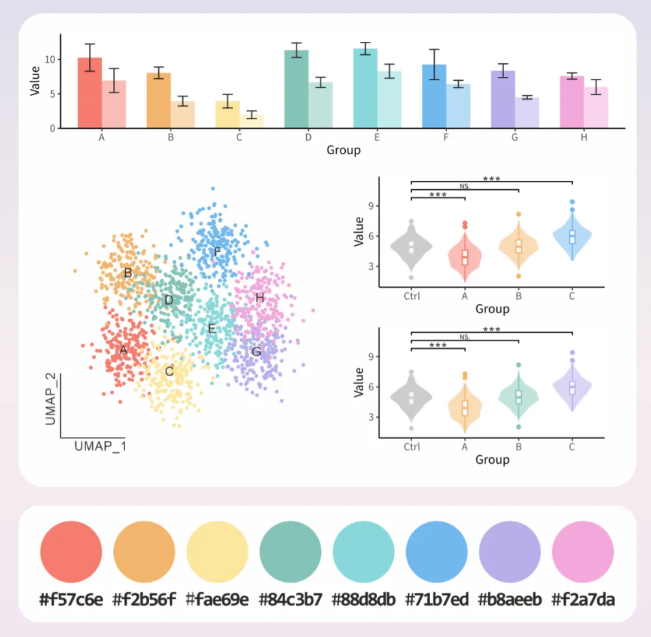
\includegraphics[width=.5\linewidth]{img202406111720.png}
    \caption{\label{fig:img202406111720}绘图配色}
\end{figure}
\subsection{Paper}
\subsection{常规MD模拟Ar与MD2结合部位以及关键残基}
\subsection{模拟关键残基突变对Ar在MD2中富集的影响}
\subsubsection{构建残基突变模拟体系进行动力学模拟}
\noindent\textbf{说明:}取先前MD模拟的最后一帧保存为pdb文件,将蛋白单独取出来使用pymol进行突变,然后使用pdb2gmx构建突变后的top文件和gro文件,然后将突变后的top文件和gro文件将水以及离子进行合并,最后提交进行MD模拟即可。
\newline\textbf{建模脚本代码:}/惰性气体氩气MD2受体/domut202406231338.sh
\subsubsection{模拟轨迹align到同一构象上pbc处理分析}
\noindent\textbf{说明:}为了比较蛋白热点残基突变之后MD2中Ar富集的影响。将蛋白残基突变之后再次模拟Ar的富集情况。为了使得突变前后能够对比,因此在轨迹分析时,以突变前的蛋白朝向作为参考,将突变后的轨迹align到突变前结构中进行Ar富集情况绘图,从而形成对比。
\newline\textbf{操作说明:}(1)根据npt之后的gro文件生成轨迹参考结构。(2)将轨迹参考结构align到突变前构象中 (3)生成align之后构象的pbc.tpr文件。 (4)对轨迹使用-pbc atom -center, -pbc whole, -fit rot+trans将轨迹align到pbc.tpr上。
\newline\textbf{具体代码:}/惰性气体氩气MD2受体/alignpbc202406231341.sh
\subsubsection{计算Ar在水盒子中的分布}
\noindent\textbf{说明:}分别计算xy,xz和yz平面内的Ar的分布概率。对比突变前后的Ar的分布概率变化从而总结出残基突变对Ar在MD2中富集的影响。
\newline\textbf{脚本:} /script/惰性气体氩气MD2受体/ densityar202403251736.py
\subsubsection{绘制Ar在水盒子中的分布热图}
\noindent\textbf{说明:}分别绘制xy,xz和yz平面内的Ar的分布热图。这里只放xy平面的代码,其余两个平面热图绘制只需在该基础上稍加修改即可。
\newline\textbf{脚本:} /script/惰性气体氩气MD2受体/ plothotmap202403252113.py
\subsection{Umbrella Sampling研究Ar对MD2-LPS结合的影响}
\subsubsection{不加Ar时MD2-LPS的Umbrella Sampling的PMF计算}
\noindent\textbf{说明:}将不加Ar的MD2-LPS的MD模拟的最后一帧结构取出,先从该结构出发进行SMD,然后进行Umbrella Sampling,进而计算PMF。
\newline\textbf{(1) 选择MD的最后一帧进行SMD}
\newline\textbf{选择MD的最后一帧保存为pdb文件}
\lstset{language=bash}
\begin{lstlisting}
gmx trjconv -f ../../prod/step5_1.gro -s ../../prod/step5_1.tpr -o step5_1.pdb -n index.ndx
\end{lstlisting}
\noindent\textbf{获得距离蛋白质心最近的原子编号:}/惰性气体氩气MD2受体/getcenter202406231343.py
\newline \textbf{获得蛋白复合物的长宽高:}/惰性气体氩气MD2受体/getxyz202406231344.py
\newline \textbf{制作朝向的index文件}
\newline \textbf{说明:}制作index.ndx将朝向的原子编号加进去。
\lstset{language=bash}
\begin{lstlisting}
gmx make_ndx -f step5_1.pdb -o index.ndx
# [ direc ]
# 2150 2385 2387 2389 2390 2472 2559
\end{lstlisting}
\noindent\textbf{建模}
\newline\textbf{说明:}在建模时候要拉的那个轴的方向要尽可能的建的长一些,该轴的长度要大于要拉的距离的两倍。跑之前注意检查mdp文件里面的位置限制。em,equil里面的都进行位置限制,pull时候只限制蛋白。
\newline 脚本如:/惰性气体氩气MD2受体/do202406231348.sh
\newline \textbf{(2) 进行Umbrella Sampling}
具体参考如下有Ar时的Umbrella Sampling代码。
\subsubsection{加Ar时MD2-LPS的Umbrella Sampling的PMF计算}
\noindent\textbf{说明:}考虑到加Ar之后的MD2-LPS的结合模式与晶体结构的MD2-LPS结合模式不一致。所以优先模拟Ar存在条件下的MD2-LPS结合模式(即将LPS拉离MD2一段距离之后,Ar在MD2口袋富集,此时再进行MD模拟获得MD2-LPS在Ar存在下的结合模式)。再从该结合模式出发进行SMD,Umbrella Sampling,进而进行PMF计算。
\newline\textbf{(1) 选择MD的最后一帧进行Ar存在时的SMD}
\newline\textbf{(2) 选择SMD中LPS拉出的3个不同距离构象进行MD寻找Ar存在下MD2-LPS结合模式}
\newline\textbf{(3) 从Ar存在下MD2-LPS的MD最后一帧进行SMD}
\newline\textbf{(4) 进行Ar存在条件下的MD2-LPS的Umbrella Sampling的PMF计算}
\newline 计算SMD过程中参考组和拉动组质心间距离:
\newline 代码如:/惰性气体氩气MD2受体/do202406231350.sh
\newline 根据质心之间的距离进行窗口分割,确定挑选的所有窗口构象的时刻点:
\newline 代码如:/惰性气体氩气MD2受体/do202406231351.py
\newline 从SMD轨迹中截取每个时刻窗口的构象准备Umbrella Sampling文件:
\newline 代码如:/惰性气体氩气MD2受体/do202406231352.sh
\newline 整合所有窗口的构象,可用于pymol查看:
\newline 代码如:/惰性气体氩气MD2受体/do202406231353.py
\newline 生成mdp文件以及提交脚本文件:
\newline 代码如:/惰性气体氩气MD2受体/do202406231354.py
\newline 提交运行
\newline 代码如:/惰性气体氩气MD2受体/do202406231355.sh
\newline wham生成PMF能量曲线文件
\newline 代码如:/惰性气体氩气MD2受体/do202406231357.sh
\newline 绘制PMF曲线
\newline 代码如:/惰性气体氩气MD2受体/do202406231358.py
\subsubsection{汇总加Ar与不加Ar时的PMF能量曲线绘图}
\noindent 选择加Ar与不加Ar时的wham生成的zerror.xvg文件作为输入,将两条曲线画在一幅图中进行对比。
\newline 根据两个zerror.xvg文件生成绘图的输入文件。
\newline 代码如:/惰性气体氩气MD2受体/do202406231404.py
\newline 绘图代码如:/惰性气体氩气MD2受体/do202406231407.py
\section{二甲双胍作用于呼吸链蛋白Cyro-EM课题}
\subsection{该课题的一些相关背景}
\noindent \textbf{= 氯胍的直构象和弯曲构象}:以前解析的晶体结构里面已经有复合物结构涉及氯胍的直构象和弯曲构象。该复合物结构的pdbid是8F4T。
\subsection{课题文件存储结构}
\noindent = /BackGround/ \# 背景相关一些琐碎的文件
\newline = /data\_from\_experiment/ \# 这个文件夹中是湿实验那边第一次发过来的没有精细分类的结构文件。
\newline = /wholesystemcutmd/ \# 这个文件夹是将第一次发的没有精细分类的结构整体结构或者裁剪之后的多种结构进行的分子动力学模拟结果文件。
\newline \indent == /wholesystemcutmd/wholesystem/ \# 这个文件夹是将整体的所有链全部进行建模MD的文件。> 200w原子。
\newline \indent == /wholesystemcutmd/Qchannelcut/ \# 这个文件夹是将整体体系进行多次切分查看模拟效率的文件。其中r1和r2是两次选取不同链的切割方式。 
\newline = /all\_10\_classes\_structures/ \# 该课题最终的大部分绘图的数据都是放置在这个文件夹中。 
\newline \indent == /all\_10\_classes\_structures/filesfromexperiment/ \# 这个文件夹中的是湿实验那边发过来的多次结构。
\newline \indent == /all\_10\_classes\_structures/simulation/ \# 二甲双胍和氯胍的所有模拟数据文件都在该文件夹中。
\newline \indent == /all\_10\_classes\_structures/simulation/MF8/nocharge/ \# 二甲双胍的数据文件,该文件夹中含有open状态时候的class1和class3的Q tunnel的PMF模拟计算。
还有close状态时候的class5的PMF计算。class5里面还含有二甲双胍周围残基的FEP计算,两种构象的二甲双胍的计算模拟以及将辅酶Q从Qtunnel中间拉到底部的PMF的模拟数据。
还有二甲双胍入膜的PMF的计算数据的PMF\_mem\_wat文件夹。由于文件夹的层次很多,所以具体的每个文件夹中都有readme.md的说明文件进行文件标注。
\newline \indent == /all\_10\_classes\_structures/simulation/PGL/ \# 氯胍的数据文件
\subsection{Figure}
\noindent \textbf{= 氯胍的一维PMF曲线绘图:}
\newline \textbf{== 处理水到膜过程时候的曲线:}将氯胍从膜的中间分别向两侧溶剂中拉动进行PMF计算。得到zerror.xvg文件。
选择一侧的PMF曲线进行处理,处理时候水里面的值应该是0,并且水里面的曲线应该趋向于平坦。x值为0的时候应该也是平的,是在膜里面。
脚本:/二甲双胍作用于呼吸链蛋白Cyro-EM课题/do202407122013.py
\newline \textbf{== 处理呼吸蛋白孔道里面的PMF曲线:}从氯胍的两个位置分别进行相对方向的拉动以及PMF计算。合并之后得到zrror\_normal\_c1.dat。
将这个文件的0点与水到膜过程时候的曲线进行拼接。脚本:/二甲双胍作用于呼吸链蛋白Cyro-EM课题/do202407122021.py
\newline \textbf{== 对水到膜以及孔道内部PMF接口处的曲线进行平滑:}首先将水到膜的PMF曲线数据和孔道内部的PMF曲线数据整合到一个文件中。
对这个文件整体进行平滑操作并生成一个新的平滑之后的文件,脚本:/二甲双胍作用于呼吸链蛋白Cyro-EM课题/plotpmf202407122056.py。
将平滑后的文件的接头部分复制进整体PMF曲线数据中。最后绘制最终的文件,脚本:/二甲双胍作用于呼吸链蛋白Cyro-EM课题/plotpmf202407122101.py。
\newline \textbf{= 氯胍的二维MetaD绘图:}
\newline \textbf{== 从multiwalker产生的多个势能文件中提取特定模拟时间的势能文件:}/二甲双胍作用于呼吸链蛋白Cyro-EM课题/Extrahills202407181643.py。
\newline \textbf{== 合并所有势能文件并使用plumed计算自由能landscape:}/二甲双胍作用于呼吸链蛋白Cyro-EM课题/posprocess202407181659.sh。
\newline \textbf{== 将生成的bias文件转换为自由能绘图数据:}/二甲双胍作用于呼吸链蛋白Cyro-EM课题/getcontourfinput202407182027.py。
\newline \textbf{== 绘制自由能landscape:}/二甲双胍作用于呼吸链蛋白Cyro-EM课题/Step12plotconsurf202407182029.py。
\newline \textbf{== 对x轴坐标进行缩放:}/二甲双胍作用于呼吸链蛋白Cyro-EM课题/scalex202407182040.py
\newline \textbf{== 对x轴坐标进行平移:}/二甲双胍作用于呼吸链蛋白Cyro-EM课题/Normalizex202407182044.py
\subsection{Paper}
\subsection{该课题使用的一些通用的技术和脚本}
\noindent = 膜蛋白建模
\newline == 将庞大的蛋白进行重新编链。
\newline\indent 大蛋白重新编链的脚本:mkrenamechainsforsupercomplex.py
\newline == 将呼吸蛋白截取通道部分结构后加膜加二甲双胍加配体上传charmmgui进行建模。
\newline\indent 先将配体在pymol中编辑完成之后保存为mol2文件。将配体mol2文件上传charmmgui配体准备模块中生成配体的参数文件.rtf和.prm。
然后将蛋白-配体复合物文件上传charmmgui中的膜体系准备模块中建模。
\newline\noindent = 膜蛋白MD模拟
\newline\indent (1) 使用charmmgui进行体系建模;(2) mdp文件:/script/mdp202404212117/ (3) 提交的脚本文件:/script/job202404212119.sh
\newline\noindent = 膜蛋白SMD
\newline\indent (1) 截取MD的最后一帧或者其中一帧进行SMD模拟;(2) mdp文件:/script/mdp202404212121 (3) 提交的脚本文件:/script/job202404212122.sh 
(4) SMD模拟轨迹可视化处理:/script/do202404212123.sh  
\newline\noindent = 膜蛋白Umbrella Sampling
\newline\indent (1) 根据SMD的结果可以重新选取CV使用gmx distance计算距离:/script/Step5 Getgrpsdistance202404212130.sh 
(2) 根据距离确定伞形采样的窗口构象:/script/Step61 Getwins202404212133.py 
(3) 生成所有采样窗口以及窗口文件:/script/Step7 Getpmffiles.sh 
(4) 生成所有窗口的可视化文件:/script/Step71 allgroscheckpymol.py 
(5) 生成mdp文件以及提交脚本文件:/script/Step81 PMFinfile.py 
(6) 续跑Umbrella Sampling脚本文件:/script/Step101 PMFxuinfile.py  
(7) 整合多次续跑的伞采样结果脚本文件:/script/Step11 Mergepullf.py 
(8) wham获得结果绘制曲线脚本文件:/script/Step12 Getresults.sh 
(9) 绘制PMF曲线:/script/Step12 Plotpmfcurve.py 
(10) 绘制histo曲线:/script/Step13 Plothistocurve.py 
(11) plotly绘制交互式histo曲线:/script/Step141 Plothistocurveplotlyinput.py
(12) 在跑完PMF之后,有的时候需要重新选定新的参考点生成新的tpr文件用于计算新的pmf曲线。脚本:newtprpmf.sh 
\subsection{对close状态中二甲双胍的两种结合构象进行MD模拟}
\noindent = 对两种状态都MD模拟
\newline\indent (1) 将实验获得的超大蛋白进行重新编号,否则不能在pymol中进行正确的可视化。
(2) 选择适当的链截取出来。
(3) 对配体U10和MF8进行编辑,保证结构的正确性,保存为mol2文件并上传charmmgui生成配体的力场文件。
(4) 将charmmgui生成的配体pdb文件贴进复合物pdb中替换原本的配体。
(5) 将复合物上传charmmgui的双层膜体系准备模块时候,遇到一个奇葩问题。也不知道是charmmgui更新了还是怎么滴的,之前用的时候
直接将辅酶Q的名字改成UQ10就可以,但是最近用的时候不行,显示top文件里面没有名称为UQ10的残基。
看了一下发现toppar\_all36\_lipid\_archaeal.str文件被去掉了。真是奇葩,不明白为什么去掉。然后试了各种方法都不太行。
所以将UQ10的末端去掉了一个甲基然后再使用ligand准备模块准备力场进行charmmgui建模,后面下载下来之后,再将完整的配体pdb和top进行替换即可。
(6) 后面的操作基本正常,没有其他。
(7) 
\subsection{对氯胍的open和close构象进行模拟研究氯胍的弯曲程度}
\noindent\textbf{= MD模拟体系构建以及模拟}
\newline (1) 将实验获得的超大蛋白进行重新编号,否则不能在pymol中进行正确的可视化。
(2) 选择适当的链截取出来。
(3) 将孔道口部和底部的氯胍分子保存为结构正确的mol2格式文件。孔道口部的分子命名为PG1,孔道底部的分子命名为PG2。
(4) 将PG1和PG2都上传到charmm-gui上使用Ligand Reader \& Modeller模块进行力场参数准备。
(5) 将PGL力场文件夹中的ligandrm.pdb文件的小分子复制进入蛋白文件中形成复合物文件。将2MR改成ARG。
(6) 将复合物文件上传charmm-gui中的Membrane Builder进行建模。
(7) 将建模文件从charmm-gui下载,有的时候可能需要修改不同的小分子力场进行模拟,比如swissparm,需要将下载下来的文件的gro文件中的小分子重新保存成mol2格式并且上传charmmgui或者其他小分子参数化方法进行小分子配体的参数建模。
并使用新生成小分子参数替换charmmgui上下载下来的itp文件以及gro文件中的坐标进行建模以及模拟。
(8) 文件替换完成之后记得使用gmx make\_ndx重新生成下index.ndx文件,进行模拟计算即可。
\newline\textbf{= 结果分析-角度计算-绘图}
\newline\textbf{== gmx计算角度:}/二甲双胍作用于呼吸链蛋白Cyro-EM课题/getangle202407221555.sh
\newline\textbf{== 绘图三次重复轨迹的曲线图:}/二甲双胍作用于呼吸链蛋白Cyro-EM课题/plot202407231535.py
\subsection{对氯胍的构象进行PMF计算}
\subsection{对氯胍在孔道里面运动时候的弯曲程度分布进行multi-walker的MetaD计算}
\noindent = MD模拟
\newline = SMD
\newline = Multi Walker MetaD
\newline == 将SMD时候的index.ndx以及topol文件复制到该文件夹中。
\newline == 根据SMD的结果使用gmx distance计算距离:./二甲双胍作用于呼吸链蛋白Cyro-EM课题/Step5 Getgrpsdistance202404212130.sh  
\newline == 根据距离确定伞形采样的窗口构象:./二甲双胍作用于呼吸链蛋白Cyro-EM课题/Step61 Getwins202404212133.py 
\newline == 生成所有采样窗口以及窗口文件:./二甲双胍作用于呼吸链蛋白Cyro-EM课题/Step7 Getpmffiles.sh 
\newline == 将每个窗口的初始pdb文件整合到一个pse文件中进行可视化。
脚本:./二甲双胍作用于呼吸链蛋白Cyro-EM课题/Step71allgroscheckpymol.py
\newline == 生成进行Multi Walker MetaD所需要的plumed文件。并且需要创建all\_walkers文件夹。
脚本:./二甲双胍作用于呼吸链蛋白Cyro-EM课题/plumedmultiwalker202406261638.py
\newline == 生成Multi Walker MetaD的脚本提交文件。
脚本:./二甲双胍作用于呼吸链蛋白Cyro-EM课题/MultiWalkerMetaD202406261643.py
\newline == 续跑Multi Walker MetaD的脚本提交文件。
脚本:./二甲双胍作用于呼吸链蛋白Cyro-EM课题/MultiWalkerMetaDxu202406271259.py
\newline == 将多个窗口整合到一个bash文件中进行提交模拟。
脚本:./二甲双胍作用于呼吸链蛋白Cyro-EM课题/PMFinfilemergesubmit202407192013.py
\subsection{将二甲双胍和氯胍进行跨膜的Umbrella Sampling}
\noindent \textbf{= PMF结果处理以及绘图}
\newline == 将三组平行的PMF结果进行合并计算三组平行结果的平均值以及误差。
脚本:./二甲双胍作用于呼吸链蛋白Cyro-EM课题/dupscommeanse202407241311.py。
\newline == 将水里面的曲线作为标准基线,设置为0。并将误差一列变成上下限的两列数据,用于绘图的输入。
脚本:./二甲双胍作用于呼吸链蛋白Cyro-EM课题/normalizationy202407241321.py。

\section{鲜味受体与多肽对接课题}
\subsection{ColabFold预测鲜味受体的三维结构}
(1) 先将序列上传至ColabFold的在线网站上生成MSA的文件(此时只需在网站上将预测模型的数目设置为0即可),然后下载多序列比对结果的压缩包。
\newline\indent (2) 将压缩包上传到128上提交下述脚本进行预测即可:~/script/鲜味受体与多肽对接课题/sub202403022353.sh
\subsection{ADCP对接鲜味受体和多肽}
\subsection{smina对接鲜味受体和多肽}
\section{r-AA肽衍生物计算模拟}
\subsection{r-AA多肽模拟的力场比较}
\noindent = 对实验方给的初始结构进行GAFF力场,CGenFF力场以及MMFF94力场的模拟比较:
\newline\indent 对实验方给的初始结构的前处理,先保存成pdb文件,然后使用脚本:/script/r-AA肽衍生物计算模拟 uniqueatomnames202403241421.py 对其原子名称进行唯一化。然后再对pdb文件的单双键进行
检查并删除重复的原子,最后保存成mol2文件去生成力场。
\newline\indent MMFF94使用的是swissparm生成力场文件,其他的使用的是AutoFF生成的力场文件。
\newline\indent gmx 计算距离。脚本:/script/r-AA肽衍生物计算模拟/ gmxdistance202403261029.sh
\newline\indent 计算概率以及计算自由能。脚本:/script/r-AA肽衍生物计算模拟/ dgmap202403261031.py
\newline\indent 绘制自由能景观图。脚本:/script/r-AA肽衍生物计算模拟/ plotdgmap202403261032.py
\subsection{实验方合成的rAA肽在MMFF94力场下的计算模拟}
\subsection{受体蛋白ASGPR的Colab建模}
\subsection{受体ASGPR与配体的计算模拟}
\noindent = ASGPR与配体晶体结构的计算模拟
\newline\noindent = 建模的带跨膜域的ASGPR三聚体与三个配体结构的计算模拟
\newline\indent 将蛋白-离子-配体的晶体结构中的蛋白align到三聚体的每个单体中,将配体和离子copy到三聚体中,
构建带有跨膜结构域的三聚体蛋白-离子-配体结构。进行多组平行的MD模拟,统计三聚体free状态下的相对排列低能量结构。
计算距离的脚本:do202404221245.sh。统计距离分布概率密度和自由能的脚本:ddgdistance202404221248.py。
绘制概率密度和自由能曲线的脚本:plot202404221326.py。找出三个能量最低点对应的具体距离数值脚本:findmin202404221637.py。 
找出能量最低构象脚本:findminenergytime202404221909.py。
\subsection{对rAA肽进行SMD模拟,固定一端,拉动另一端,对rAA肽两端距离采样}
\section{辐射分子相似性查找-张连学}
\subsection{与ZINC中化合物进行相似性比对-拓扑比对}
\noindent (1) 将ZINC中的所有SMILES均分成100份:do202405091015.sh 
\newline\noindent (2) 将一个分子与分成100份的ZINC使用拓扑结构比较方法进行相似性比较:do202405091020.py do202405091031.py do202405091100.sh
\subsection{与ZINC中化合物进行相似性比对-MACCS比对}
\noindent (1) 将一个分子与分成100份的ZINC使用MACCS比较方法进行相似性比较:do202405091426.py do202405091031.py do202405091100.sh
\subsection{与ChemDiv中化合物进行相似性比对-拓扑比对}
\subsection{与ChemDiv中化合物进行相似性比对-MACCS比对}
\section{浙一白雪莉老师合作的Serpinb9相关课题}
\subsection{Figures}
\subsection{Paper}
\noindent 写作文章参考:Inhibition of DEF-p65 Interactions as a Potential Avenue to Suppress Tumor Growth in Pancreatic Cancer  
\subsection{对Serpinb9界面部位关键残基的FEP计算-Gromacs}
\noindent = 体系准备的总体脚本:./Serpinb9/Dutopolsetup202406301122.sh
\newline = 准备lambda的mdp文件的脚本:./Serpinb9/mkFEPlambdamdp202406301124.py
\newline = 多个副本之间交换的FEP提交脚本:./Serpinb9/job202406301129.parrallel
\newline = 单个文件MD的FEP提交脚本:./Serpinb9/mksubmitfepwinsGromacs202406301132.py
\newline = FEP跑完之后计算ddg的脚本:./Serpinb9/mkgetFEPresultgmx202406301133.sh
\subsection{将SMS与设计的多肽1-5进行MD和MM/GBSA计算}
\noindent = 对复合物进行MD计算:体系准备脚本:syssetup202407022106.sh;产生mdp文件的脚本:Step2generatemdp202407022115.py;
产生提交文件的脚本:Step3generatesubmitsh202407022119.py
\newline = MD之后的pbc处理,聚类,RMSD计算的脚本见:/Serpinb9/pbc202406161024.sh
\section{申有青老师HA-OP课题(做不了一点,送xf)}
\subsection{模拟50HA和40HA10OP的全原子}
\noindent\textbf{(1) 50HA的模拟建模}:有晶体结构,晶体结构中只有4个重复单元,但是需要构建13个重复单元的结构,所以在pymol中进行编辑构建。
上传到attoff中产生力场文件。
\noindent\textbf{(2) 50HA在真空中模拟}:采一些构象进行构建含有50个HA的初始结构。

如果你在Overleaf上编译本~\cite{zjuthesisrules}模板,请注意如下事项:

\begin{itemize}
    \item 删除根目录的 ``.latexmkrc'' 文件,否则编译失败且不报任何错误
    \item 字体有版权所以本模板不能附带字体,请务必手动上传字体文件,并在各个专业模板下手动指定字体。
        具体方法参照 GitHub 主页的说明。
    \item 当前的Overleaf默认使用TexLive 2017进行编译,但一些伪粗体复制乱码的问题需要TexLive 2019版本来解决。
        所以各位同学可以在Overleaf上编写论文时务必切换到TexLive 2019或更新版本来编译,以免产生查重相关问题。
        具体说明参照 GitHub 主页。
\end{itemize}


\section{节标题}

我们可以用includegraphics来插入现有的jpg等格式的图片,
如\autoref{fig:zju-logo}所示。

\begin{figure}[htbp]
    \centering
    
\includegraphics[width=.3\linewidth]{logo/zju}
    \caption{\label{fig:zju-logo}浙江大学LOGO}
\end{figure}


\subsection{小节标题}


\par 如\autoref{tab:sample}所示,这是一张自动调节列宽的表格。

\begin{table}[htbp]
    \caption{\label{tab:sample}自动调节列宽的表格}
    \begin{tabularx}{\linewidth}{c|X<{\centering}}
        \hline
        第一列 & 第二列 \\ \hline
        xxx & xxx \\ \hline
        xxx & xxx \\ \hline
        xxx & xxx \\ \hline
    \end{tabularx}
\end{table}


\par 如\autoref{equ:sample},这是一个公式

\begin{equation}
    \label{equ:sample}
    A=\overbrace{(a+b+c)+\underbrace{i(d+e+f)}_{\text{虚数}}}^{\text{复数}}
\end{equation}

\chapter{另一章}


\begin{figure}[htbp]
    \centering
    \includegraphics[width=.3\linewidth]{example-image-a}
    \caption{\label{fig:fig-placeholder}图片占位符}
\end{figure}

\chapter{再一章}

\par 如\autoref{alg:sample},这是一个算法

\begin{algorithm}[H]
    \begin{algorithmic} % enter the algorithmic environment
        \REQUIRE $n \geq 0 \vee x \neq 0$
        \ENSURE $y = x^n$
        \STATE $y \Leftarrow 1$
        \IF{$n < 0$}
            \STATE $X \Leftarrow 1 / x$
            \STATE $N \Leftarrow -n$
        \ELSE
            \STATE $X \Leftarrow x$
            \STATE $N \Leftarrow n$
        \ENDIF
        \WHILE{$N \neq 0$}
            \IF{$N$ is even}
                \STATE $X \Leftarrow X \times X$
                \STATE $N \Leftarrow N / 2$
            \ELSE[$N$ is odd]
                \STATE $y \Leftarrow y \times X$
                \STATE $N \Leftarrow N - 1$
            \ENDIF
        \ENDWHILE
    \end{algorithmic}
    \caption{\label{alg:sample}算法样例}
\end{algorithm}


ttt